\graphicspath{{sec01/images/}{sec01/code/}}
\lstset{inputpath=sec01/code/}


\section{Очень продвинутый \LaTeX: программирование и работа с примитивами}

\begin{frame}[fragile]{Соглашение о наименовании}\relax
    \begin{itemize}
             \item Если команда сделана для пользователей, используется короткое имя и lowcase: \ccol\section, \ccol\emph\ and \ccol\times
             \item Если команда для создателей других пакетов, используется CamelCase: \ccol\InputIfFileExists\ \ccol\RequirePackage\  \ccol\PassOptionsToClass
             \item Для ``приватных'' команд используется @. Большая часть внутренних команд \LaTeX а использует эту букву внутри: \ccol{\@tempcnta}, \ccol{\@ifnextchar}, \ccol{\@eha}. \\ Чтобы использовать такие команды внутри файлов .tex, это использование надо окружить \ccol\makeatletter, <use command>, \ccol\makeatother
    \end{itemize}
          
\end{frame}

\begin{frame}\relax

{\centering\Huge \TeX\ это Тьюринг полный язык программирования

}
\cscfootnote{
\url{https://stackoverflow.com/questions/2968411/ive-heard-that-latex-is-turing-complete-are-there-any-programs-written-in-late} 
\overC{https://www.overleaf.com/learn/latex/Articles/LaTeX_is_More_Powerful_than_you_Think_-_Computing_the_Fibonacci_Numbers_and_Turing_Completeness} 
\url{http://sdh33b.blogspot.com/2008/07/icfp-contest-2008.html}}
     
\end{frame}

\subsection{Создание команд}

\begin{frame}[fragile]{Создание команд \tW}\relax
    В \TeX\ для создания команд используется \ccol\def.

    \twocolImg{
    \lstinputlisting[linerange={8-9, 14-16}]{commandwith.tex}
    }{commandwith}
    
        {\footnotesize
     \begin{tabbing}
     
        \rulecommand{1}\lstinline|\def|\= \rulecommand{2}\lstinline|\dfdx| \= \rulecommand{3}\lstinline|#1| \= \rulecommand{4}\lstinline|#2| \= \rulecommand{5}\lstinline|{\frac{\partial #1}{\partial #2}|\\
        \footnotesize  команда задания макроса  \> \>  \>  \> \\
        \>  имя макроса \> \>  \> \\
         \> \>\footnotesize первый аргумент  \>  \> \\
         \> \>  \> \footnotesize  второй аргумент  \> \\
         \> \>  \>  \>\footnotesize  что делать с аргументами \\
        
    \end{tabbing}}
    \cscfootnote{\tugC{https://www.tug.org/utilities/plain/cseq.html\#def-rp} \knuthc{20}[209]}
\end{frame}

\outclassframe{
\begin{frame}{Создание команд \tW}\relax
    \small Используйте префикс \ccol\global, чтобы макрос был доступен вне стандартной области видимости. 
    
    И \ccol\long\ чтобы его частями могли стать несколько параграфов.
    
    
\end{frame}
}

{\def\parseLine#1, #2\par{arg1: '\texttt{#1}' arg2: '\texttt{#2}'}
\begin{frame}[fragile]{Pattern matching\tW}\relax
    Зачем нужно писать \lstinline|\def\name#1#2#3|... вместо чего-то наподобие \LaTeX, \lstinline|\def\name[5]|\inpause
    
    Ради таких штук:
    % \lstset
    % {
    %     basicstyle=\tt\normalsize,
    % }
    \footnotesize
     \begin{tabbing}
     
        \lstinline|\def\parseLine |\= \lstinline|#1| \= \lstinline|, | \= \lstinline|#2| \= \lstinline|\par| \= \lstinline|{arg1: #1, arg2: #2}|\kill
        \lstinline|\def\parseLine |\> \rulecommand{1}\lstinline|#1| \> \rulecommand{2}\lstinline|, | \> \rulecommand{3}\lstinline|#2| \> \rulecommand{4}\lstinline|\par| \> \rulecommand{5}\lstinline|{arg1: '#1' arg2: '#2'}|\\
        \>\footnotesize  начинает собирать первый аргумент \> \>  \>  \> \\
        \> \>\tiny  первый аргумент -- всё до ближайшей запятой с пробелом \> \>  \> \\
        \> \> \>\footnotesize  начинает собирать второй аргумент  \>  \> \\
        \> \> \>  \> \footnotesize  всё до нового параграфа  \> \\
        \> \> \>  \>  \>\footnotesize  что делать с аргументами \\
        
    \end{tabbing}\vspace*{-2ex}
    \lstinline|\parseLine Hello ,,, World| выдаст \parseLine Hello ,,, World
    
\end{frame}

}
\lookCode{Мы часто можем ссылаться на ГитХаб. Давайте напишем команду, что сокращала бы такую ссылку

{\centering
\includegraphics[width=0.7\textwidth]{09_pattern.png}\par}\pause
\begin{enumerate}
    \item Перенесём иконку ГитХаба в рабочую папку
    \item Создадим команду, которая преобразует \url{https://github.com/Lavton/latexLectures} в \url{/latexLectures}
    \item Создадим обёртку над командой, которая бы добавляла иконку гитхаба 
     
\end{enumerate}
}

\inclassframe{
    \begin{frame}{Пора добавить динамики в отображение!}\relax Условные операторы\end{frame}
}
%%%%%%%%%%%%%%%%%%%%%%%% условия %%%%%%%%%%%%%%%%%%%%%%%%%%%%%%%%%%%%%%%%%%%%%%%%%%%%%%
\subsection{Условные операторы}

\begin{frame}[fragile]{Сравнить строки(макросы)\tW}\relax

    \twocolImg{
    \lstinputlisting[linerange={12-21}]{ifmy.tex}
    }{ifmy}   

    \footnotesize
    {\ccsc \verb|\ifx\<first>\<second>  <code1>  [\else  <code2>]  \fi|}
    
\end{frame}

\begin{frame}[fragile]{Сравнить числа\tW}\relax
    
    \footnotesize
     \begin{tabbing} 
        \lstinline|\ifnum |\= \rulecommand{1}\lstinline|\year > 2022 |\= \rulecommand{2}\footnotesize как дела, потомки? \= \rulecommand{3}\lstinline|\else | \= \rulecommand{4}\footnotesize свеженькая лекция! \= \lstinline|\fi|\\ 
        \>\footnotesize условие \> \> \> \> \\
        \> \>\footnotesize что происходит при прохождении условия? \> \> \> \\
        \> \>  \>\footnotesize опциональный блок \textit{else} \> \> \\
        \> \>  \> \>\scriptsize что при провале условия \> \\
    
    \end{tabbing}
    \vspace*{-2ex}
    
    Кстати, \ifnum\year>2022 как дела, потомки?\else свеженькая лекция!\fi 
    
    \cscfootnote{Ещё можно использовать {\ccol\ifodd} чтобы сравнить на чётность}
    
\end{frame}

\begin{frame}[fragile]{``именнованные'' условия: \ccol\newif\tW}\relax
    \samePosPicture{newifmy}{12-20}  

    \outclasshigh{Т.е. сначала мы объявляем, что хотим использовать условие под таким вот именем. Потом -- определяем, сейчас это true или false.

    И где-то, где уже реализуется логика, код выполняется в зависимости от того, считается ли \textit{В данный момент} условие истинным или ложным. Что мы задали раньше.}
    \cscfootnote{\url{http://handyfloss.net/2007.08/latex-programming-how-to-implement-conditionals/}}
\end{frame}

\cprotect\outclassframe{
\begin{frame}[fragile]{Проверка мод\tW}\relax

    \begin{itemize}
        \item {\ccol\ifmmode} это математическая мода?
        \item {\ccol\ifvmode} это вертикальная мода?
        \item {\ccol\ifhmode} это горизонтальная мода?
        \item {\ccol\ifinner} это одна из следующих мод: internal vertical mode, restricted horizontal mode, (nondisplay) mathmode?
         
    \end{itemize}
    
    \cprotect\cscfootnote{остальные ``if''ы могут быть найдены в \knuthc{20}[221]. Например \ccol\ifdim\ проверяет длины, \ccol\ifeof\ -- конец файла, \ccol\ifcsname\ -- существование команды по имени\\
    Ещё полезна инверсия бывает: \lstinline|\def\ifnot#1{#1\else\expandafter\expandafter\fi\iffalse\iftrue\fi}| (\stExC{https://tex.stackexchange.com/questions/108911/negating-ifeof})}
\end{frame}
}


\begin{frame}[fragile]{Условия в \LaTeX: \ccol\ifthenelse\lW}\relax
    \lstinline|\usepackage{ifthen}|
        \vspace*{-2ex}
        
    \footnotesize
     \begin{tabbing}
     
        \lstinline|\ifthenelse |\= \rulecommand{1}\lstinline|{\equal{aa}{bb}}|\= \rulecommand{2}\lstinline|{world is mad}| \= \rulecommand{3}\lstinline|{world is good}|\\ 
        \>\footnotesize проверка условия для строк. Для чисел можно >, <,.. \> \> \\
        \> \> \footnotesize что делать если условие прошло\> \\
        \> \> \> \footnotesize что делать если условие\\
        \> \> \> ~~~~~~~~~~ провалилось\\
    
    \end{tabbing}    \vspace*{-8ex}
        
    
      \cscfootnote{Ещё есть хороший пакет xstring. Там проверка строк, подстрок, операции с ними...\\ А проверить pdfLaTeX, XeLaTeX и LuaTeX можно с \stExC{https://tex.stackexchange.com/questions/47576/combining-ifxetex-and-ifluatex-with-the-logical-or-operation}}
\end{frame}

\lookCode{Уберём номер слайда с титульника, подвинем линейку к заголовку (когда нет подзаголовка)\inpause

Вдруг у нас есть проблема: посчитать количество ``сложных'' слайдов. Как это сделать?
}

\subsection{Работа с примитивами}
%%%%%%%%%%%%%%%%%%%%%%%%%%%%%%%%%%%%%% примитивы %%%%%%%%%%%%%%%%%%%%%
%%%%%%%%%%%%%% счётчики %%%%%%%%%
\begin{frame}{Счётчики -- counters}\relax

    Счётчик -- просто целое число. Но используется он в огромном числе вариантов.
    
    Номер раздела, слайда, уравнения, цитаты, нумерованный список и многое другое.
     
    Например 
    \begin{itemize}
        \item номер этого слайда - \ccol\insertframenumber = \insertframenumber
        \item номер страницы при этом -- \ccol\the\ccol\count0 = \ccol\thepage = \thepage
         
    \end{itemize}
\end{frame}

\begin{frame}[fragile]{Определение и манипулирование счётчиками\lW}\relax
    \begin{itemize}
        \item \lstinline|\newcounter{abcd}| -- объявить счётчик 
        \item \lstinline|\setcounter{abcd}{2022}| -- присвоить счётчику значение
        \item \lstinline|\addtocounter{abcd}{-42}| -- добавить число
         
    \end{itemize}
     
\end{frame}
\newcounter{tmptt}
     \newcommand{\countab}[1]{
     \ccol#1\{countname\}&
     \setcounter{tmptt}{1} #1{tmptt} &
     \setcounter{tmptt}{2} #1{tmptt} &
     \setcounter{tmptt}{3} #1{tmptt} &
     \setcounter{tmptt}{4} #1{tmptt} &
     \setcounter{tmptt}{5} #1{tmptt} &
     \setcounter{tmptt}{6} #1{tmptt} &
     \setcounter{tmptt}{7} #1{tmptt} &
     \setcounter{tmptt}{8} #1{tmptt} &
     \setcounter{tmptt}{9} #1{tmptt}
     \\}

\outclassframe{
\begin{frame}{Отображение счётчиков\lW}\relax
     
     \footnotesize
     \begin{tabular}{l|ccccccccc}
          \countab{\arabic}
          \countab{\alph}
          \countab{\Alph}
          \countab{\roman}
          \countab{\Roman}
          \countab{\fnsymbol}
     \end{tabular}
     \vspace{1ex}
     
     \cscfootnote{ \wikiC{https://en.wikibooks.org/wiki/LaTeX/Counters\#Counter_style} \lmanc{13.1}[126]\\ 
     см \lvoc{IX.2.3}[295] для нашего аналога \ccol\alph}
\end{frame}
}

\begin{frame}{Доминирование счётчиков\lW\magicPage}\relax
    ``Доминирование'' одного счётчика над другим -- значит при обновлении первого счётчика второй вернётся к 1.
    
    Доминирование -- механизм, благодаря которому все подразделы могут иметь нумерацию, привязанную к разделу, а не сквозную. 
    
     
\end{frame}

\begin{frame}[fragile]{Добавить доминирование счётчику\magicPage}\relax

    \newcommand{\modif}[3]{\fbox{\parbox{\textwidth}{\makebox[\textwidth]{\small\makebox[0.25\textwidth]{\tiny #1}\hfill$\to$\hfill\makebox[0.55\textwidth]{\tiny #2}}\\ #3}}}
    
    \centering
    \modif{\string\newcounter\{task\}}{\ocol\newcounter\{task\}[section]}{\ocol\newcounter\{<slave>\}[<master>] обнулит значение <slave> при изменеии <master>}
    
    
    \modif{\ccol\addtocounter\{task\}\{1\}}{\ccol\refstepcounter\{task\}}{
    Используйте \ccol\refstepcounter\{<counter>\}, чтобы правильно работал механизм ссылок
    }
    
    
    % \modif{\string\textbf\{Task \string\#\string\arabic\{task\}\}.}{\tiny\string\textbf\{Task \string\#\string\arabic\{section\}.\string\arabic\{task\}\}.}{Внутри \string\newcommand\{\string\tsk\} to redefine the labels}
    
    
    \modif{}{\tiny\string\renewcommand\{\ccol\thetask\}\{\string\arabic\{section\}.\string\arabic\{task\}\}}{Переопределите \string\renewcommand\{\ccol{\the<counter>}\}, чтобы правильно работали ссылки \ccol\ref}
    
    \cscfootnote{\lvoc{VII.3.3}[250] \lmanc{13.6}[128]}
\end{frame}

\begin{frame}[fragile]{Счётчики в \TeX}\relax
    \begin{itemize}
        \item \textbf{Определить свой} \ccol\newcount\ccol{\<countname>} как \verb|\newcount\mycounter|
        \item \textbf{Задать значение} \ccol{\<countname>=<number>}  Или используйте \ccol\countdef. Как \footnotesize\verb|\countdef\mynumber=43|
        \item \textbf{Добавить число}  \ccol{\advance\string\<countname>\ by <number>}. Так же можно использовать \ccol\multiply\ и \ccol\divide. \begin{itemize}
            \item\footnotesize Эти команды меняют значение счётчика, к которому приложены
            \item\footnotesize Просто арифметическую операцию можно сделать с помощью \ccol\numexpr: \verb|\numexpr 4*3-\the\count0=| \the\numexpr 4*3-\the\count0\relax
        \end{itemize}
        \item \textbf{Показать значение} \ccol{\the\string\<countname>} или \ccol\number\ или \ccol\romannumeral
         
    \end{itemize}
     
     
     \cscfootnote{\knuthc{15}[129] \stExC{https://tex.stackexchange.com/questions/245635/formal-syntax-rules-of-dimexpr-numexpr-glueexpr}\\В реальности используется \ccol\count<number> (Как \ccol\count212). Что делает \ccol\newcount, это ищет не занятое число и предоставляет его по имени.}
     
\end{frame}
\lookCode{Добавим индикатор, что слайд ``сложный'' и выведем число таких сложных слайдов\pause

Вопрос: как бы сделать, чтобы для слайдов 16:9 заметки внизу могли быть шире, чем для 4:3?
}

%%%%%%%%%%%%%%%%%%%%%%%%%%%% длины 

\begin{frame}{Длины -- lenghts}\relax
    Длина -- число + размерность. В реальности кратное ``scaled points'' = $1/2^{16}$pt.
    
    Длины тоже можно прибавлять, умножать, делить... Причём размерность приведётся.
\end{frame}

\begin{frame}{Манипулирование длиной в \LaTeX\lW}\relax

    \begin{itemize}
        \item \textbf{Определить длину} \ccol{\newlength\{\textbackslash<lenname>\}}
        \item \textbf{Задать длину} \ccol{\setlength}
        \item \textbf{Добавить что-то к длине}  \ccol{\addtolength}
        \item \textbf{Отобразить длину} \ccol{\the\textbackslash<lenname>}. Но ещё можно использовать \ncol\usepackage{printlen}\ и потом \ccol\uselengthunit, \ccol\printlength
         
    \end{itemize}
    
    \cscfootnote{\wikiC{https://en.wikibooks.org/wiki/LaTeX/Lengths} }
\end{frame}

\begin{frame}[fragile]{Манипулирование длиной в \TeX\tW}\relax
    \begin{itemize}
        \item \textbf{Определить длину} \ccol{\newdimen\textbackslash<lenname>}
        \item \textbf{Задать длину} {\ccsc\textbackslash<lenname>=<len>}
        \item \textbf{Добавить к длине}  \ccol{\advance\textbackslash<lenname>\ by <len>}. Ещё есть \ccol\multiply\ и \ccol\divide. \\И \ccol\dimexp, работающая по аналогии с \verb|\numexpr|.
        \item \textbf{Показать длину} \ccol{\the\textbackslash<lenname>}
    \end{itemize}
    
    \cscfootnote{\knuthc{15}[132]. Для клея есть отдельный \ccol\glueexpr }
\end{frame}
\lookCode{Вынесем ширину footnote в отдельную переменную. И заодно длину линии по верху. \pause

    А теперь определим ширину в зависимости от ширины слайда.\pause
    \begin{enumerate}
        \item Введём переменную со значениями 0, 1. Она отвечает за то, ``широк'' ли слайд 
        \item В зависимости от значения переменной присвоим длине заметки 9 или 12 cm
         
    \end{enumerate} \pause

    Проблема: у нас бывают очень большие заметки внизу. Было бы здорово, если заметка очень уж большая, расположить её по всему низу, убрав номер слайда и лого.
}

%%%%%%%%%%%%%%%%%%%%%%% БОКСЫ
\begin{frame}{Боксы -- boxes}\relax
    Боксы -- прямоугольники, по которым \TeX\ определяет положение объектов.
    
    Боксы можно сохранять в память (без печати), узнавать ширину-высоту-глубину, печатать
         
\end{frame}


\begin{frame}[fragile]{Манипулирование боксом в \LaTeX\lW\magicPage}\relax
    \begin{itemize}
        \item \textbf{Определить бокс} \ccol{\newsavebox\{\string\<boxname>\}}
        \item \textbf{Задать бокс} \ccol{\savebox} (\lstinline|\savebox{\mybox}{\hbox{LaTeX content}}|)
        \item \textbf{Напечатать содержимое не удаляя бокс:} \ccol{\usebox} (\lstinline|\usebox{\mybox}|)
        \item \textbf{Узнать размеры}: 
        \begin{enumerate}
            \item Создать переменную длины: \ccol\newlength
            \item Определить переменную одним из измерений боксов:
            \begin{itemize}
                \item ширина: \verb|\settowidth{\<len-var>}{\usebox{\<box>}}|
                \item высота: \verb|\settoheight{\<len-var>}{\usebox{\<box>}}|
                \item глубина: \verb|\settodepth{\<len-var>}{\usebox{\<box>}}|
            \end{itemize}
        \end{enumerate}
    \end{itemize}

    \cscfootnote{\lmanc{14.4-6}[133] \lmanc{20.5, 20.7}[183]}
\end{frame}


\begin{frame}[fragile]{Манипулирование боксом в \TeX\tW\magicPage}\relax
    \begin{itemize}
        \item \textbf{Определить бокс} \ccol{\newbox\string\<boxname>}
        \item \textbf{Задать бокс} \ccol{\setbox\string\<boxname>=<box>} (\lstinline|\setbox\mybox=\hbox{LaTeX content}|)
        \item \textbf{Напечатать содержимое не удаляя бокс:} \ccol{\copy\string\<boxname>}
        \item \textbf{Напечатать содержимое и удалить бокс из памяти:} \ccol{\box\string\<boxname>}
        \item \textbf{Узнать размеры}: ширина: \ccol\wd, высота: \ccol\ht, глубина: \ccol\dp\ ~~ (\lstinline|\dp\mybox|)
         
    \end{itemize}

    \cscfootnote{\knuthc{15}[131]. Ещё существуют \ccol\unhbox, \ccol\unvbox, \ccol\unhcopy, \ccol\unvcopy. Их задача -- прикрепить содержимое бокса с текущему списку без изменений }
\end{frame}

\outclassframe{
\begin{frame}{Остальные примитивы \TeX\magicPage}\relax
    В дополнение к длинам, боксам и счётчикам в \TeX\ есть:
    \begin{itemize}
        \item \ccol\skip, \ccol\muskip\ -- регистры для клея в обычной и математической моде соответственно
        \item \ccol\toks\ -- регистры для строк 
         
    \end{itemize}
     
\end{frame}
}

\lookCode{Сделаем, чтобы широкая заметка могла занять весь ``подвал''. И тогда она займёт не так много места по вертикали

{\centering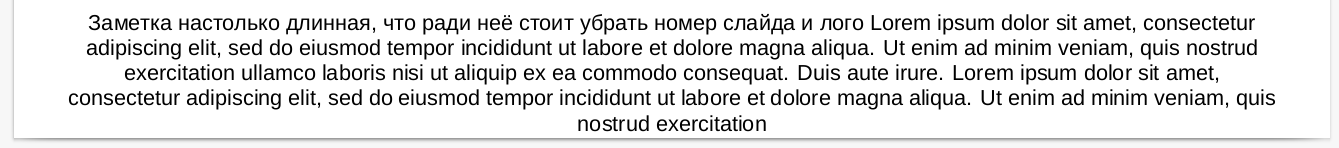
\includegraphics[width=0.7\textwidth]{13_box.png}\par}\pause
\begin{enumerate}
    \item Зададим новый бокс, в котором будет храниться заметка
    \item Создадим функцию, которая бы проверила -- выше ли заметка некого порога 
    \item Создадим именованный if, значение которого бы показывало -- нужно нам заметку расширять на весь слайд или нет 
    \item В footline проверим значение if-а и или расширим заметку или нет 
     
\end{enumerate}
}
\inclassframe{
    \begin{frame}{Мы почти у финиша!}
        Итак, мы умеем делать уже почти всё. Одно лишь загадка: как сделать прогрессбар?\inpause

        ... для него нужны циклы, рекурсия и даже работа с файловой системой!
    \end{frame}
}

%%%%%%%%%%%%%%%%%%%%%%%%%%%%%%%%%% рекурсия и циклы
\subsection{Циклы и рекурсия}
\begin{frame}[fragile]{Циклы \outclasshigh{и рекурсия }в \TeX \tW\magicPage}\relax
    Циклы:\vspace*{-2ex}
    
    \samePosPicture{loopmy}{12-17} \vspace*{-1ex}
    
    \cprotect\outclasshigh{\ccol\loop\ для старта, <code> внутри, потом один из операторов серии {\ccsc\verb|\if<..>|}, ещё код <code>, заканчиваем \ccol\repeat\ (вместо \ccol\fi).
    
    рекурсия:
    \vspace*{-2ex}
    
    \samePosPicture{reqmy}{12-13}}

    \cprotect\cscfootnote{\knuthc{20}[228].\\ \ccol\loop\ это просто \lstinline|\def\loop#1\repeat{\def\body{#1}\iterate}|,\\ а \ccol\iterate: 
    \lstinline|\def\iterate{\body\let\next=\iterate\else\let\next=\relax\fi\next}|}
     
\end{frame}

\begin{frame}[fragile]{Циклы в \LaTeX\lW\magicPage}\relax
     \twocolImg{
    \lstinputlisting[linerange={8-8, 13-16}]{forloopmy.tex}
    }{forloopmy}
    \ncol \usepackage{forloop}
    
    \cprotect\outclasshigh{\twocolImg{
    \lstinputlisting[linerange={8-8, 13-15}]{foreachmy.tex}
    }{foreachmy}
    
    \ncol \usepackage{pgffor}, часть пакета pgf, часть TikZ}
    
    \cscfootnote{\url{https://stackoverflow.com/questions/2561791/iteration-in-latex}}
\end{frame}

%%%%%%%%%%%%%%%%%%%%%%%%%%%%%%%%%%%% работа с ФС
\subsection{Работа с файловой системой}
\begin{frame}[fragile]{Запись в ФС}\relax
     \lstset
    {
        basicstyle=\tt\normalsize,
    }
    \begin{itemize}
        \item \ccol\newrite\ объявляет переменную: \lstinline|\newwrite\myfile|. 
        \item \ccol\openout\ открывает файл на запись: \lstinline|\openout\myfile=outfile.txt|.
        \begin{itemize}
            \item Можно использовать \ccol\jobname\ в качестве имени файла.
        \end{itemize} 
        \item \ccol\write<register>\ собственно производит запись: \lstinline|\write\myfile{{\noexpand\bf Hello}\World}|
        \outclass{\begin{itemize}
            \item \outclasshigh{\ccol\noexpand\ тут не даёт команде запуститься, а просто записывает её (см также \ccol\expandafter)}
        \end{itemize}}
        \item \ccol\closeout\ закрывает файл на запись: \lstinline|\closeout\myfile|
    \end{itemize}
    
    \cscfootnote{Как и со всеми регистрами, можно использовать просто число: например \ccol\write4}
     
\end{frame}
\begin{frame}[fragile]{Чтение из ФС}\relax
     \lstset
    {
        basicstyle=\tt\normalsize,
    }
    \begin{itemize}
        \item \ccol\newread\ объявляет переменную: \lstinline|\newread\myfile|.
        \item \ccol\openin\ открывает файл на чтение:  \lstinline|\openin\myfile=infile.txt|.
        \item \ccol\read<register>\ \ccol{to}\string\<newvariable> собственно читает в перменную: \lstinline|\read\myfile to\myline|
        \item \ccol\ifeof\ проверяет, достигли ли мы конца файла: \lstinline|\ifeof\myfile|
        \item \ccol\closein\ закрывает файл на чтение: \lstinline|\closein\myfile|
    \end{itemize}
\end{frame}

\begin{frame}[fragile]{Работа с командной строкой\magicPage}\relax
    \footnotesize
    \begin{tabbing} 
        \rulecommand{1}\lstinline|\immediate|\= \rulecommand{2}\lstinline|\write18|\= \rulecommand{3}\lstinline|{wget https://<url>.png -O image.png}|\\ 
        \footnotesize запустить команду сразу как увидим \tiny(иначе запуск при формировании страницы) \> \> \\ 
        \> \footnotesize запись в 18 регистр = в командную строку \> \\
        \> \> \footnotesize текст команды \\ 
    \end{tabbing}

    \cprotect\outclasshigh{При компиляции из командной строки надо использовать ключи \verb|--enable-write18 -interaction=nonstopmode|}
\end{frame}

\begin{frame}{\LaTeX\ и предсказание будущего}\relax

\TeX\ читает код последовательно. \TeX\ знает лишь о той части кода, которая уже прочитана на момент отрисовки данной страницы.\\

Все перекрёстные ссылки, любая информация с ``будущих страниц'' требует запись этой информации в файл и чтение при новом запуске.

Вот почему \LaTeX\ так часто надо запускать 2 раза.
    
\end{frame}

%%%%%%%%%%%%%%%%%%%%%%%%%%%%%%%%%%% имена команд 
\subsection{Манипулирование с именами команд и ещё несколько ключевых слов}
\begin{frame}[fragile]{\ccol\let\magicPage}\relax
     \lstset
    {
        basicstyle=\tt\normalsize,
    }
    \ccol\let\ Позволяет копировать описание макроса в новое имя. После этого старое можно переназначить:
    \begin{itemize}
        \item \lstinline|\def\a{hello}  \let\b=\a| назначит \ccol\b\ слово ``hello''.
        \item \lstinline|\def\a{\b\ world}  \a| выведет ``hello world''
    \end{itemize}
    
\end{frame}

\begin{frame}[fragile]{Expansion\magicPage}\relax
     % \lstset
    % {
        % basicstyle=\tt\normalsize,
    % }
    \footnotesize
    \begin{itemize}
        \item \ccol\expandafter\ говорит, что сначала должно выполнится содержимое команды, а лишь потом сама команда.
        \begin{itemize}
            \item \lstinline|\def\a{ooo}    \uppercase{\a, my oborona}| вернёт ``ooo, MY OBORONA''
            \item \lstinline|\def\a{ooo}    \uppercase\expandafter{\a, my oborona}| вернёт ``OOO, MY OBORONA''
        \end{itemize}
        \item \ccol\edef\ полностью раскроет все макросы внутри
        \begin{itemize}
            \item \lstinline|\def\testp{\thepage}| всегда будет возвращать текущую страницу
            \item \lstinline|\edef\testp{\thepage}| всегда будет возвращать страницу, на которой объявили макрос
        \end{itemize}
        
    \end{itemize}
    \cscfootnote{\overC{https://www.overleaf.com/learn/latex/Articles/How_does_\%5Cexpandafter_work\%3A_The_meaning_of_expansion} \overC{https://www.overleaf.com/learn/latex/Articles/How_does_\%5Cexpandafter_work\%3A_From_basic_principles_to_exploring_TeX\%27s_source_code}
    \stExC{https://tex.stackexchange.com/questions/451/when-to-use-edef-noexpand-and-expandafter}
    }
     
\end{frame}
{\def\myfontchange#1{\csname text#1\endcsname}
\begin{frame}[fragile]{Манипулирование именами команд\magicPage}\relax
     \lstset
    {
        basicstyle=\tt\normalsize,
    }
    \begin{itemize}
        \item Написать \lstinline|\csname textit\endcsname| всё равно, что написать команду \string\textit: \lstinline|\csname textit\endcsname{my text}| даст \csname textit\endcsname{my text}
        \item \lstinline|\string\textit| вернёт просто \string\textit
    \end{itemize}\pause
    
    Пример использования:
    \begin{itemize}
    \item Зададим команду \lstinline|\def\myfontchange#1{\csname text#1\endcsname}|
    \item \lstinline|\myfontchange{it}{hello}| даст \myfontchange{it}{hello}
    \item \lstinline|\myfontchange{bf}{world}| даст \myfontchange{bf}{world}
    \end{itemize}
\end{frame}

}
\begin{frame}[fragile]{Catcodes\magicPage}{что отвечает за комментарий, а что -- символ команды?}\relax
\catcode`?=14
    \footnotesize
    \begin{tabbing}
     
        \rulecommand{1}\lstinline|\catcode`|\= \rulecommand{2}\lstinline|\%|\= = \= \rulecommand{3}12\\ 
        Меняем категорию символа\> \> \> \\
        \> Символ -- \%. Раньше отвечал за комментарий \> \> \\
        \> \> \> новый код символа -- 12. Обычный текст\\
        \> \> \> \tiny 14 -- код комментария, 1 -- начало группы (\{), и т.д...
    
    \end{tabbing}  \vspace{-0.5cm}
    
    \samePosPicture{catcodesmy}{12-20}
    
    \cscfootnote{\wikiCC{https://en.wikibooks.org/wiki/TeX/catcode}}
\end{frame}

%%%%%%%%%%%%%%%%%%%%%%%%%%%%%%%%%% debug
\subsection{Дебаггинг и логгирование}
\begin{frame}{Способы дебаггинга}\relax
    В \TeX\ можно вывести интересующую информацию в лог-файл. Есть три способа это сделать:
    \begin{itemize}
        \item {\ccsc show-команды} -- выводят в лог раскрытие конкретного макроса или содержимое конкретного примитива 
        \item {\ccsc tracing-команды} -- меняют уровень логгирования, позволяя заглянуть внутрь всей работы
        \item \ccol\message\ -- просто что-то вывести в лог         
    \end{itemize}
     
\end{frame}
\begin{frame}{Show-команды\magicPage}{Использование: \ccol\show\ccol\macros}\relax
    \small
    \begin{description}
        \item[\ccol{\show}] логгирует, что внутри макроса
        \item[\ccol\showthe] логгирует содержимое счётчика или длины 
        \outclass{\item[\ccol\showbox] \outclasshigh{логгирует содержимое бокса (какой там клей, какие слова, etc)
        \begin{description}
            \item[\ccol\showboxdepth] показывает глубину вложенности бокса
            \item[\ccol\showboxbreadth] сколько элементов на этом уровне
        \end{description}
        \item[\ccol\showlists] описывает контент списка боксов во всех 4х нематематических режимах
        \item[\ccol\showhyphens\{Word\}] показывает возможные переносы слова Word.}}
    \end{description}
     \cscfootnote{\stExC{https://tex.stackexchange.com/questions/364942/show-family-debugging-commands}}
\end{frame}
\begin{frame}{tracing-команды\magicPage}{Использование: \ccol{\tracingmacros=1} <что-то> \ccol{\tracingmacros=0}}\relax
     \footnotesize Если >0, пишет в лог-файл...

    \begin{description}
        \item[\ccol\tracingcommands] команды
        \item[\ccol\tracingmacros] раскрытие макросов и их аргументов
        \item[\ccol\tracingpages] стоимость расчёта страницы
        \outclass{\item[\ccol\tracinglostchars] \outclasshigh{каких символов нет в текущем шрифте
        \item[\ccol\tracingonline] пишет и в терминал и в лог
        \item[\ccol\tracingoutput] содержимое боксов
        \item[\ccol\tracingparagraphs] сводку по расчёту переноса строк
        \item[\ccol\tracingrestores] save-stack
        \item[\ccol\tracingstats] статистику использования памяти
        \item[\ccol\tracingall] абсолютно всё из вышеперечисленного}}
    \end{description}
         \cscfootnote{\stExC{https://tex.stackexchange.com/questions/60491/latex-tracing-commands-list}}
\end{frame}
\begin{frame}{\ccol\message\ и \ccol\typeout}\relax
    Пишет сообщение в лог:
    \begin{itemize}
        \item \ccol{\message\{<msg>\}} -- \TeX-command
        \item \ccol{\typeout\{<msg>\}} -- \LaTeX-command
    \end{itemize}
     
\end{frame}

\cprotect\outclassframe{
\begin{frame}[fragile]{P.S. нотация шрифтов}\relax
     Иногда вы можете увидеть подобный ворнинг в лог-файле:
     {\ccsc LaTeX Font Warning: Font shape `T1/calligra/bx/n' undefined}. Как читать такое обозначение?
     \centering 
    \begin{tabular}{c|c|c|c|c}
    T1&calligra&bx&n&\\ 
    OT1&cmr&m&it&10\\\hline
    \large encoding & font family & series & shape & font size
    \end{tabular}
    
    Подробнее см. ``fntguide''. 
    \cscfootnote{\normalfont \url{https://mirror.macomnet.net/pub/CTAN/macros/latex/base/fntguide.pdf}: 2.1, \normalfont\url{https://mirror.macomnet.net/pub/CTAN/macros/latex/base/encguide.pdf}}
\end{frame}
}

\lookCode{На этом теория закончилась. Пора применить все знания и создать прогрессбар!}

\begin{frame}{Что сегодня узнали}\relax
    \begin{enumerate}
        \item Примитивы в \LaTeX
        \begin{enumerate}
            \item Как \TeX\ видит наш документ: боксы и клей
            \item Какие примитивы существуют: длины, счётчики и другое
            \item Как манипулировать примитивами
        \end{enumerate}
        
        \item Программирование в \TeX\ и \LaTeX
        \begin{enumerate}
            \item Создание макросов
            \item Условные операторы
            \item Циклы и рекурсия
            \item Операции ввода-вывода
            \item Отладка
        \end{enumerate}
         
    \end{enumerate}
\end{frame}

\begin{frame}{Что сегодня сделали}\relax
    \begin{itemize}
        \item Создали шаблон с нуля
        \item Научились создавать свои команды и работать с параметрами шаблонов
        \item Сделали красивый футер: расположили заметку по центру, выставили пробелы, научились расширять пространство для заметки
        \item Построили прогрессбар, привязанной к секции
    \end{itemize}
    
\end{frame}